\externaldocument{clendshape_classification}
\externaldocument{lit_review}

\chapter{Audio Driven Blendshape GAN} \label{chap:generation}
This chapter shall discuss the use of GANs for audio driven facial animation.
Unlike previous generative models which solve a regression problem to correctly match an audio input to a sequence of parameters which describe facial motion, GANs also include an noise input resulting in variations in the output from the same conditional input.
The model outputs will then be assessed on the classification models discussed in Chapter \ref{chap:classification}.
The GAN is comprised of two neural networks, a Generator and a Critic, which are trained together using the outputs of each network to train the other.

\section{Problem Definition}
Currently, there is a lack of 3D temporal datasets which sync speech audio with corresponding facial motion with the purpose of training a model for VSR.
Such datasets are difficult to capture directly due to the equipment and time required.
Similar datasets exist which have enabled for the creation of audio driven models but these datasets are limited in size and variation and have led to models which are specific to subjects either though direct subject specific training data as with the model by Karras et al. \cite{Karras2017a} or through character encoding, as is the case with the VOCA model \cite{Cudeiro2019}.
Through the use of these models, a synthetic dataset of 3D temporal facial motion was generated as described in Section \ref{sec:dataset_gen}.
This data however is subject to all biases and restrictions the VOCA model is subject to.
An appropriate dataset would contain a small vocabulary, similar to the LRW dataset of 500 words, all spoken by multiple subjects to capture different speaking styles for the same words captured from `\textit{in the wild}' scenarios.

An appropriate dataset would meet the following conditions:
\begin{itemize}
    \item A small vocabulary of a similar size to the LRW dataset.
    \item Multiple subjects speaking the same vocabulary to capture different speaking styles for the same words.
    \item ``\textit{In the wild}'' audio conditions.
\end{itemize}

As a means to increase the variation in speaking style in existing audio drive generative models such as VOCA, a GAN model is to be trained on the data generated by the VOCA model and the original LRW audio from which the VOCA generated dataset was driven from.
The resulting generative model should be able to replicate the results of the VOCA model, but with increased variation in speaking styles due to the noise input component.

\section{Model Inputs}
The generative model is to be driven from an audio input of audio samples from the LRW dataset which were used as inputs to the VOCA model to generate the dataset of Blendshape Parameters.
Audio data in the time domain has a high number of samples per second to allow all frequencies observable by human hearing to be captured.
Human hearing can commonly hear up to 20kHz, which results in a sample rate of at least 40kHz to meet the Nyquist sampling rate, which states that the sample rate must be at least twice the desired maximum observable frequency to accurately represent the signal at this frequency.
40,000 samples for a single second is however, is a large number of samples and an inefficient data representation.
Commonly audio data is converted to the frequency domain which allows for a far more efficient means of data representation. 

\subsection{Mel-frequency Cepstral Coefficients}
Common implementations of machine learning models which use audio as in input, focused on speech, have used Mel-frequency cepstral coefficients (MFCCs) to represent audio, \cite{Holmberg2006, Milner2007, Murty2006}.
MFCCs were inspired by human anatomy and speech, invented by Davis and Mermelstein in 1980 \cite{Davis1980}.
Human speech is naturally filtered by the shape of the mouth and vocal tract.
This envelope can be well represented by the short time power spectrum.
A large amount of information is contained within an audio sample in the time domain, much of which does not contain meaningful information.
By filtering the audio sample in the frequency domain to this envelope, information useful to speech detection is maintained while other information is discarded.

The first assumption is that over a short time frame, the audio signal does not statistically vary greatly.
This assumption allows the signal to be split into short frames which can be processed separately.
An example of the audio frames is show in Figure \ref{fig:mfcc_audio_frames}.

\begin{figure}[h!]
    \centering
        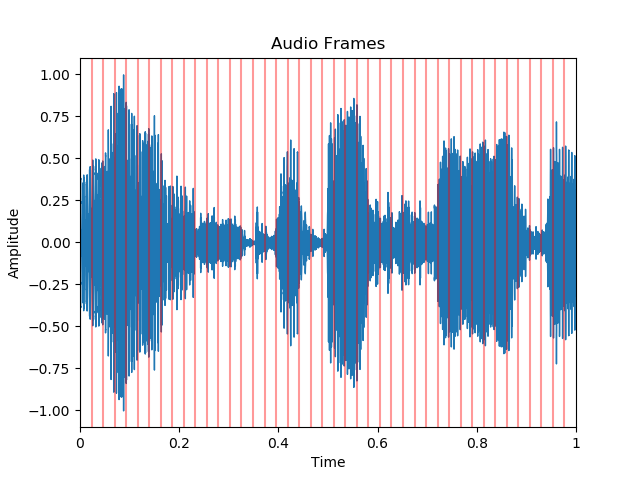
\includegraphics[width=0.7\textwidth]{figures/mfcc/audio_frames.png}
    \caption{Audio Sample Frames}\label{fig:mfcc_audio_frames}
\end{figure} 

For each frame the power spectrum is calculated using the periodogram estimation.  
The incentive behind calculating the power spectrum is derived from human anatomy, specifically from the cochlea.
The cochlea is a bone which resides within the ear and different parts of the bone vibrate depending on the frequency of the incoming audio signal.
The periodogram estimation of the power spectrum performs a similar operation by identifying which frequencies are present within an audio signal.
This representation still retains information which is not useful for speech recognition, for example the cochlea cannot distinguish between closely spaced frequency values, this is more apparent at higher frequencies.
The power spectrum for a single audio frame is shown in Figure \ref{fig:mfcc_power_spec}.
For this reason a series of Mel filterbanks are applied to the power spectrum and the resulting bin for each filter is summed, this gives an approximation of the energy present in each frequency region.
The Mel filterbanks are visualised in Figure \ref{fig:mfcc_mel_filterbanks}.
The log of each summation is then taken as humans do not perceive loudness on a linear scale, so the log compression matches the features more closely to what humans hear, shown in Figure \ref{fig:mfcc_log_sum}.

\begin{figure}[h!]
    \centering
    \begin{subfigure}[b]{0.49\textwidth}
        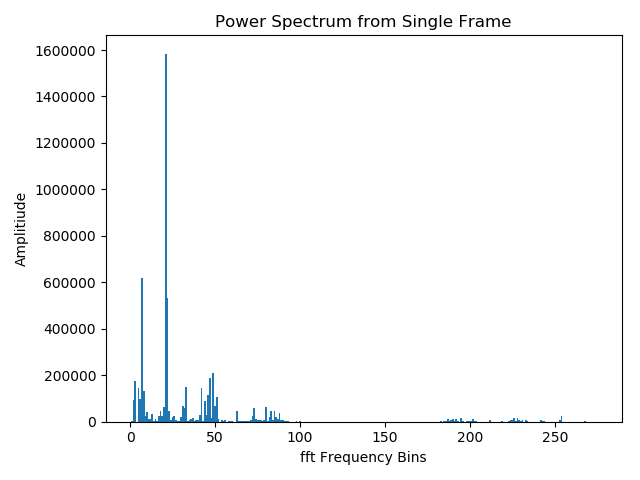
\includegraphics[width=\textwidth]{figures/mfcc/frame_power_spectrum.png}
        \caption{Audio Frame Power Spectrum}\label{fig:mfcc_power_spec}
    \end{subfigure}
    \begin{subfigure}[b]{0.49\textwidth}
        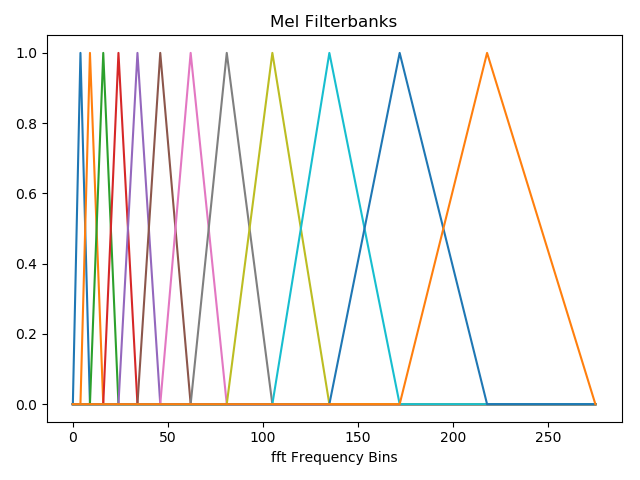
\includegraphics[width=\textwidth]{figures/mfcc/filterbanks.png}
        \caption{Mel Filterbanks}\label{fig:mfcc_mel_filterbanks}
    \end{subfigure}
    \caption{Mel Filterbank Processing}\label{fig:mfcc_filterbank_processing}
\end{figure}

Lastly, the Discrete Cosine Transformation is applied to each filterbank energy, this is performed to decorrelate the filterbanks as they are highly correlated due to the overlap in the Mel filters, the resulting representation is shown in Figure \ref{fig:mfcc_dct}.
This represents the MFCC values for a single audio frame for 8 Mel filterbanks.

\begin{figure}[h!]
    \centering
    \begin{subfigure}[b]{0.49\textwidth}
        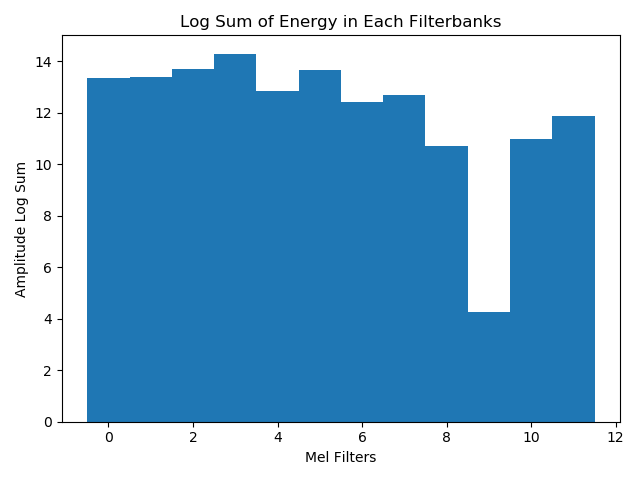
\includegraphics[width=\textwidth]{figures/mfcc/filterbank_log_sum.png}
        \caption{Log Sum}\label{fig:mfcc_log_sum}
    \end{subfigure}
    \begin{subfigure}[b]{0.49\textwidth}
        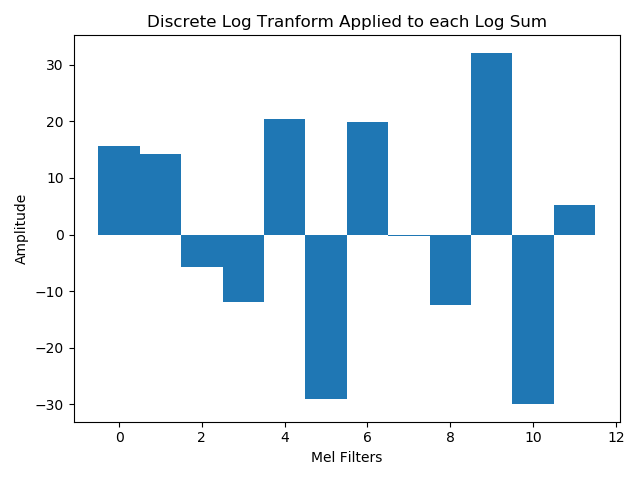
\includegraphics[width=\textwidth]{figures/mfcc/dct_applied.png}
        \caption{Discrete Cosine Transformation}\label{fig:mfcc_dct}
    \end{subfigure}
    \caption{Discrete Cosine Transformation Processing}\label{fig:mfcc_filterbank_processing}
\end{figure}

The model inputs use a total of 12 filterbanks over the span of one second audio clips.
This results in a model input MFCC $\mat{x} \in \mathbb{R}^{12 \times 43}$, visualised in Figure \ref{fig:mfcc_model_input}.

\begin{figure}[h!]
    \centering
    \begin{subfigure}[b]{0.49\textwidth}
        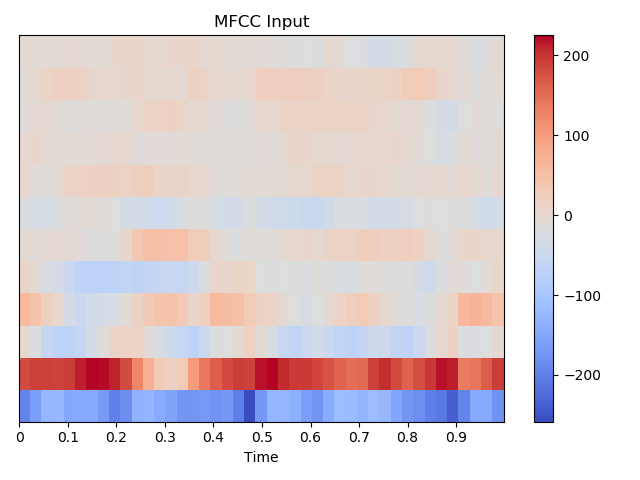
\includegraphics[width=\textwidth]{figures/mfcc/mfcc_input.png}
        \caption{MFCC Model Input}\label{fig:mfcc_input}
    \end{subfigure}
    \begin{subfigure}[b]{0.49\textwidth}
        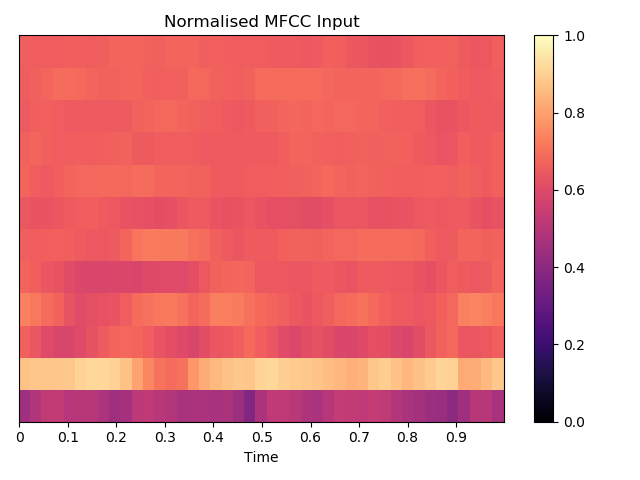
\includegraphics[width=\textwidth]{figures/mfcc/norm_mfcc_input.png}
        \caption{Normalised MFCC Model Input}\label{fig:mfcc_norm_input}
    \end{subfigure}
    \caption{MFCC Model Input}\label{fig:mfcc_model_input}
\end{figure}

\subsection{Blendshape Inputs}
The Generator aims to produce realistic Blendshape Parameters for the input audio signal, thus the input to the Critic must be the true Blendshape Parameter values and the `fake' generated Blendshape Parameters.
These values are the same as were input to the Blendshape Classification models discussed in Section \ref{sec:classification_inputs}: $\mat{y} \in \mathbb{R}^{4 \times 43}$.
The reader is directed to this section for further details.

\subsection{Noise Input}
In addition to audio represented in the form of MFCCs, the Generator is also input with a noise component consisting of random samples taken from a uniform probability distribution within the range of 0 and 1, expressed by equation (\ref{eq:uniform_dist}).

\begin{equation}\label{eq:uniform_dist}
    f(x)=\begin{cases}
      \frac{1}{b-a}, & \text{for $a \leq x \leq b$}\\
      0, & \text{elsewhere}
    \end{cases}
\end{equation}

\section{Data Preprocessing}
As with the classification models, data inputs to the model are normalised within the range [0,1], the normalised MFCC input is shown in Figure \ref{fig:mfcc_norm_input}.
This normalisation makes training both the critic and the generator easier as the range of values which the model will observe is reduced while preserving the statistical properties of the data.
As the generated Blendshape Parameters are within the range [0,1] the Sigmoid activation function can be used at the output layer of the model, rather than a linear output with an infinite range.

\section{Assessment of Model Performance} \label{sec:gan_assessment}
Assessing the performance of a GAN is less straightforward than other machine learning models.
For example, in a supervised learning scenario, a classification model can be assessed on the accuracy of predictions or f-score on a test set in addition to the model loss on these predictions, as discussed in Section \ref{sec:class_assessment}.
As GANs describe an unsupervised learning scenario, assessment metrics are less clear and problem specific.
In this problem, the aim of the Generator is to find a mapping from an audio signal represented by a series of MFCCs, to a series of Blendshape Parameters which the Critic considers to be a correct match.
The Critic's goal is to be able to judge pairings of MFCCs and Blendshape Parameters as a realistic match.

A realistic pairing of audio and Blendshape Parameters would meet the following conditions:
\begin{itemize}
    \item Movement would appear realistic to a human observer.
    \item Movement would appear correlated to the speech in the audio signal to a human observer.
    \item Speech would be correlated, such that a pretrained Blendshape classifier would be able to make some degree of successful predictions from the parameters.
\end{itemize}

The first two conditions are difficult to evaluate in a quantitative manner as this is a matter of opinion from the observer.
A subjective evaluation can be conducted on a collection of participants, however finding subjects who can accurately lip read is challenging due to the difficulty of the skill, especially in this scenario where there is no context for the spoken phrases.
Subjects who cannot lip read could be used, however this is unreliable as in many cases a video clip which has been dubbed over with an audio signal, which has been roughly matched with a speaking subject may seem plausible.
With the absence of audio, the 'realism' of the animation movement is also difficult to determine.
While aspects of animation which easily make generated data identifiable are sudden movements and shaking in the animation which would not be apparent in real speech, a series of parameter values which produce a smooth animation may easily fool observers.

A quantitative metric which can be evaluated is the performance of generated samples on the pretrained Blendshape classifiers, the architecture and performance of which is discussed in Chapter \ref{chap:classification}.
As the Generator aims to find the mapping between the input audio signal and Blendshape Parameters, if successful, the generated Blendshape Parameters should have properties similar to those of the original data which would allow for correct classification.

Given that the success of the Generator is dependent upon producing Blendshape Parameters which the critic cannot distinguish from real samples, the primary metric which shall be used is the losses on the validation set from both the Critic and the Generator during training.
Training of the Generator will be complete when the Critic can no longer distinguish between real and fake samples.
When this occurs the Critic losses have settled at 0.

\section{Model Architecture}
The GAN is composed of a Generator and a Critic, trained with the Wasserstein Loss with Gradient Penalty to ensure the Lipschtiz condition, described by equations (\ref{eq:wgan}, \ref{eq:wgan_gp}) respectively for the two models.
More details on the loss function is discussed are Section \ref{sec:Stability_to_GANs}.

\subsection{Model Structure}
The GAN model is constructed of two CNN architectures; a Generator and a Critic.
A high level diagram of the GAN model is shown by Figure \ref{fig:gan_model}.

\begin{figure}[h!]
    \centering
        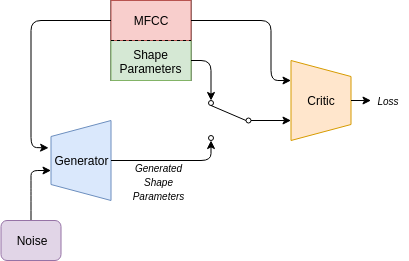
\includegraphics[width=0.9\textwidth]{figures/gan/gan.png}
    \caption{GAN Model}\label{fig:gan_model}
\end{figure} 

The Critic is trained on a corresponding pair of MFCC values and Blendshape Parameters.
The goal of the Critic is to be able to identify a correct pairing from the dataset and a false pairing consisting of MFCC values and a fake series of Blendshape Parameters generated by the Generator.
The Critic returns a score value within the range of [-1, 1], where data inputs which it regards as realistic are larger, while pairings which it regards as fake are smaller.
For each minibatch in a training epoch the Critic is shown a batch of real data values $\mat{x}$ and the Generator creates a batch of fake data values $\mat{\tilde{x}}$.
The Critic evaluates this data and returns a score for both the real and fake data.
In addition to the loss from the Critic score on real and fake data samples, the gradient penalty term is calculated, this term is to be minimised to meet the Lipschtiz condition, \cite{Gulrajani2017}.
This is found by evaluating the score of the Critic on a new data sample taken at random along the interpolation between the real and fake Blendshape Parameters, $\mat{\hat{x}}$.
The gradient penalty term $\mat{k}$ can then be found with equation (\ref{eq:grad_penalty}) with the interpolated value, where $\lambda$ is a tunable hyperparameter.

\begin{equation}\label{eq:grad_penalty}
    \mat{k} = \lambda \E{\bm{\hat{x}} \sim \Pd{\bm{\hat{x}}}} 
            [(\| \nabla_{\bm{\hat{x}}} D(\bm{\hat{x}}) \| - 1)^2]
\end{equation}

The Generator takes inputs of MFCC values and noise from a uniform distribution, these are concatenated together and processed as a single input.
The Generator then attempts to map this input into Blendshape Parameter values which the Critic evaluated to a low loss value. 
During training, the samples produced by the Generator are assessed by the Critic.
The Generator aims to have the samples it produces labelled as realistic, such that the Critic returns a high value.

At any point for the Generator to improve the quality of the samples it can produce, the Critic must initially be able to distinguish between the real and fake samples, else the Generator has no incentive to improve further.
For this reason, the Critic is trained more frequently then the Generator, in this case the Generator is trained one in ten batches, while the Critic is trained on every batch, the data is shuffled so that the Generator is still exposed to the whole training dataset.

\begin{table}[h!]
\centering
    \begin{tabular}{l | r | r}
    & \textbf{Generator} & \textbf{Critic}\\
    \hline
    Optimisation Algorithm & RMSprop & RMSprop \\
    Learning Rate          & 0.00001 & 0.00001 \\
    Scheduler              & 0.999   & 0.999   \\
    Batch Size             & 128     & 128     \\
    Training Ratio         & 1:10    & 1:1     \\
    Gradient Penalty       & -       & 5       \\
    \end{tabular} 
    \caption{GAN Hyperparameters}\label{table:gan_hyperparameters}
\end{table}

\subsection{Generator}
The Generator aims to transform noise from a uniform distribution into realistic Blendshape Parameters given the conditional input of MFCC values for a given audio sample.
Five channels of noise are sampled with the same shape as in MFCC input and the two are concatenated along the channel dimension, such that the input data is $\mat{z} \in \mathbb{R}^{6 \times 12 \times 43}$.
The Generator model architecture is a fully convolutional network which takes the input values $\mat{z}$ and transforms this into Blendshape Parameters $\mat{\tilde{x}} \in \mathbb{R}^{4 \times 43}$.

\begin{figure}[h!]
    \centering
        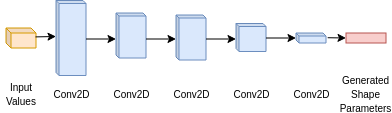
\includegraphics[width=0.8\textwidth]{figures/gan/generator.png}
    \caption{Generator Model Architecture}\label{fig:gan_gen_arch}
\end{figure}

The model (shown in Figure \ref{fig:gan_gen_arch}) consists of five convolutional layers, the detailed specification of which is shown in Table \ref{table:gan_gen_arch}.
The first pads the input along the time domain as the output dimension along the time domain is to be the same as in input, corresponding to separate frames of Blendshape Parameters, without padding this dimension would be reduced due to convolution operations.
This is a significant amount of padding to be applied to a single layer, however when a padding values of one was applied to all layers this resulted artifacts at the beginning and end of the generated sequence.
The first layer has a high number of filter channels to extract the largest possible amount of information from the input data, following layers reduce the number of channels to compress this information into the final output layer which has 4 channels, one for each Blendshape Parameter.

The model uses ReLU activate functions for all hidden layers and the Sigmoid activation function at the output layer to achieve Blendshape Parameters in the range [0, 1].
The output layer also uses a larger kernel size than the hidden layers, which all use a kernel size of 3.
When a small kernel was used at the output layer there existed a large amount of jitter in the output parameters, increasing the output kernel seems to eliminate this and produce animation with smoother motion.
The role of this output layer is not to extract useful information for subsequent layers to use, but to generate the output values.
A larger kernel increases the receptive field of this layer on the feature maps from the previous layer, resulting in reduced variation between subsequent frames and less jitter.

\begin{table}[h!]
\centering
    \begin{tabular}{ l | r | r | r | l}
    \textbf{Layer} & \textbf{Output} & \textbf{Kernel} & \textbf{Padding} & \textbf{Activation} \\ \hline
    Conv2D & 256x10x53 & (3,3) & (0,6) & ReLU    \\ \hline
    Conv2D & 128x8x51  & (3,3) & (0,0) & ReLU    \\ \hline
    Conv2D & 128x6x49  & (3,3) & (0,0) & ReLU    \\ \hline
    Conv2D & 64x4x47   & (3,3) & (0,0) & ReLU    \\ \hline
    Conv2D & 4x1x43    & (4,5) & (0,0) & Sigmoid 
    \end{tabular} 
    \caption{Generator Model Architecture}\label{table:gan_gen_arch}
\end{table}

\subsection{Critic}
The Critic aims to distinguish real data samples from the training dataset from data samples from the Generator.
The high level overview of the model architecture is shown in Figure \ref{fig:gan_critic_arch} and listed in detail in Table \ref{table:gan_critic_arch}.
Inputs to the Critic are comprised of MFCC values and Blendshape Parameters, both of which have different dimension sizes, but share a common time dimension. 
There are 12 MFCC filter values and 4 Blendshape Parameter per time instance.
In order to concatenate these values together, the Blendshape Parameter values are treated as a separate channel and duplicated 12 times, such that the Blendshape Parameters are expressed as $\mat{b} \in \mathbb{R}^{4 \times 12 \times 43}$.
This is then concatenated with the MFCC values $\mat{m} \in \mathbb{R}^{1 \times 12 \times 43}$, into the input values $\mat{x} \in \mathbb{R}^{5 \times 12 \times 43}$.

\begin{figure}[h!]
    \centering
        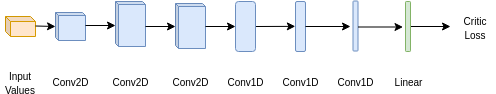
\includegraphics[width=0.9\textwidth]{figures/gan/critic.png}
    \caption{Critic Architecture}\label{fig:gan_critic_arch}
\end{figure}

The Critic model consists of three sections, the first two are built of convolutional layers using the LeakyReLU activation function while the last output layer, a linear layer using the Tanh activation function.
The first three layers are two dimensional convolutional layers which do not convolve over the time domain, just the height dimension.
This allows the model to find an efficient encoding of the input audio and Blendshape Parameters.
The number of filters is increased throughout this encoding stage as opposed to extracting a large number of filters initially as was the case with the Generator.
The reasoning behind this is that the initial input contains a great deal of repetition due to the Blendshape Parameters being duplicated into the same shape as the MFCC values.

The second section aims to convolve over the time domain, as the singleton dimension can now be collapsed, one dimension convolutional layers can now be used to achieve this.
The section consists of three convolutional layers, each of which have a stride of two and a decreasing kernel size across the three layers.
The first layer uses a kernel size of 5 in order to capture higher level features while the subsequent layers have kernel sizes of 4 and 3 respectively to capture more fine detailed features.
The final layer is a fully connected layer, which provides the critic score for the input data sample.
The layer uses the Tanh activation function to output a score in the range of [-1, 1].

\begin{table}[h!]
\centering
    \begin{tabular}{ l | r | r | r | l}
    \textbf{Layer} & \textbf{Output} & \textbf{Kernel} & \textbf{Stride} & \textbf{Activation} \\ \hline
    Conv2D & 64x5x43   & (4,1) & (1,1) & LeakyReLU \\ \hline
    Conv2D & 128x3x43  & (3,1) & (1,1) & LeakyReLU \\ \hline
    Conv2D & 128x1x43  & (3,1) & (1,1) & LeakyReLU \\ \hline
    Conv1D & 128x20    & 5     & 2     & LeakyReLU \\ \hline
    Conv1D & 128x9     & 4     & 2     & LeakyReLU \\ \hline
    Conv1D & 64x4      & 3     & 2     & LeakyReLU \\ \hline
    Linear & 16        & -     & -     & Tanh      
    \end{tabular} 
    \caption{Critic Model Architecture}\label{table:gan_critic_arch}
\end{table}

\section{Discussion of Results}
Examining the training losses of the Generator and Critic, the performance of the model can be deduced.
The first condition of the Critic is that the Lipschtiz condition is met, enforced by the gradient penalty term, by examining Figure \ref{fig:gan_critic_gp} this can be seen to reduce rapidly and remain close to zero throughout training.

\begin{figure}[h!]
    \centering
        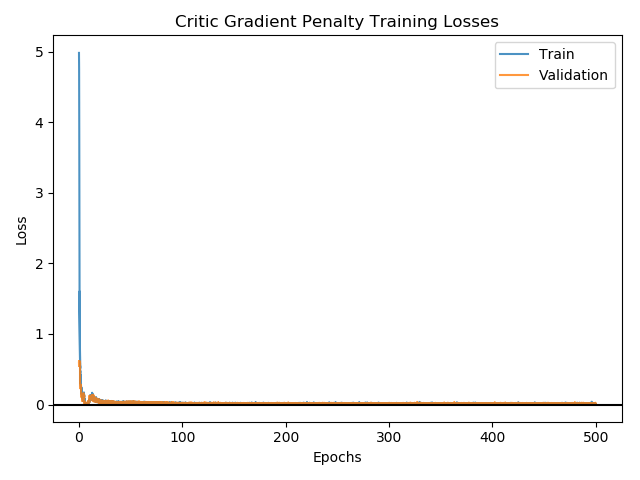
\includegraphics[width=0.65\textwidth]{figures/gan/critic_gp_train_losses.png}
    \caption{Critic Gradient Penalty Training Loss}\label{fig:gan_critic_gp}
\end{figure} 

Secondly, the total losses of the Critic as described by equation (\ref{eq:wgan_gp}) are shown in Figure \ref{fig:gan_total_critic_losses}.
Due to the high initial value of the gradient penalty term, the initial terms have not been plotted for this or subsequent plots to aid visualisation.
The Generator and Critic both aim to have as low a loss as possible, a negative Generator loss is an indication that the fake samples are being scored incorrectly by the Critic as it considers the fake Blendshape Parameters as a correct pairing for the incoming MFCC values, as described by equation (\ref{eq:wgan}).
A negative values for the total loss of the Critic is an indication that on average the real data samples are being given a higher score than the fake samples.
However, as the loss from the Critic is a summation of multiple terms, this plot alone does not display all information about the model.
From Figure \ref{fig:gan_total_critic_losses} it can be seen that throughout the whole training process the Critic correctly scores real and fake input data.

\begin{figure}[h!]
    \centering
        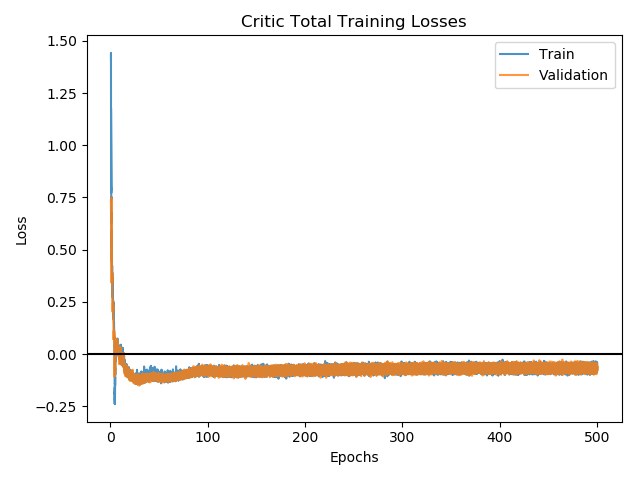
\includegraphics[width=0.7\textwidth]{figures/gan/critic_total_train_losses.png}
    \caption{Critic Total Training Losses}\label{fig:gan_total_critic_losses}
\end{figure} 

In order to gain a better insight of the Critic and Generator's training losses, the loss on the real and fake data samples can be plotted during the training process.
The Critic aims to score real samples positively and fake samples negatively, such that the total loss will be negative.
From equation (\ref{eq:wgan_gp}) the first term $\E{\bm{\tilde{x}} \sim \Pd{g}} [D(\tilde{{\bm{x}}})]$ describes how the Critic evaluates fake data samples produced by the Generator, this is plotted in Figure \ref{fig:gan_critic_fake}.
The Generator training losses are also plotted in Figure \ref{fig:gen_train_losses} and can be seen to be a mirror of the Critic's evaluation of generated samples.
From the two plots the Generator can be seen to be gradually improving throughout training, although the the losses never completely fool the Critic.
The Critic settles on a consistent loss for real data samples shown in Figure \ref{fig:gan_critic_real} as described by the second term in equation (\ref{eq:wgan_gp}): $- \E{\bm{x} \sim \Pd{r}} [D(\bm{x})]$.

\begin{figure}[h!]
    \centering
    \begin{subfigure}[b]{0.49\textwidth}
        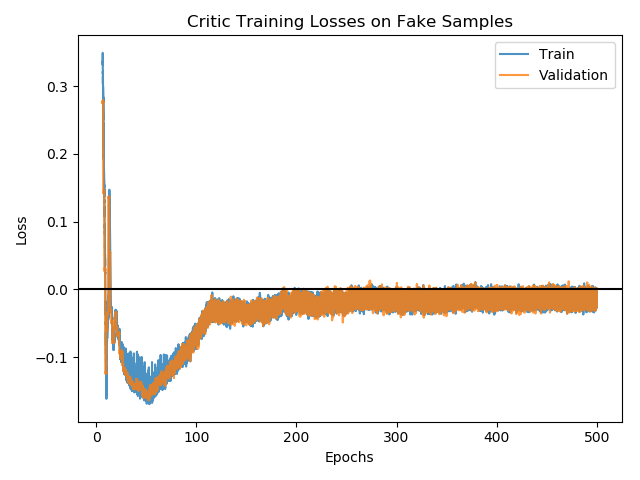
\includegraphics[width=\textwidth]{figures/gan/critic_fake_train_losses.png}
        \caption{Fake Data Samples}\label{fig:gan_critic_fake}
    \end{subfigure}
    \begin{subfigure}[b]{0.49\textwidth}
        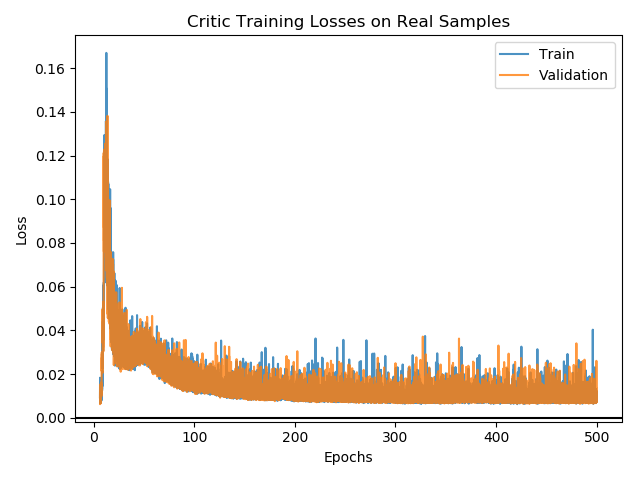
\includegraphics[width=\textwidth]{figures/gan/critic_real_train_losses.png}
        \caption{Real Data Samples}\label{fig:gan_critic_real}
    \end{subfigure}
    \caption{Training Losses from Critic for Real and Fake Data Samples}\label{fig:gan_real_fake_train_losses}
\end{figure}

\begin{figure}[h!]
    \centering
        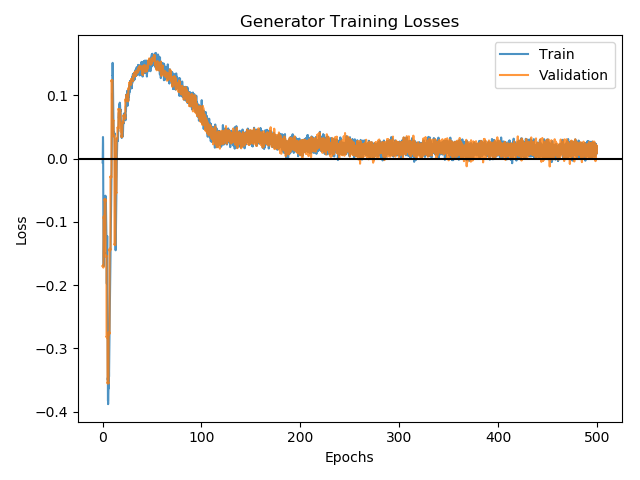
\includegraphics[width=0.7\textwidth]{figures/gan/gen_train_losses.png}
    \caption{Generator Training Losses}\label{fig:gen_train_losses}
\end{figure} 

Training settles on the Critic being able to distinguish real samples from fake, although the confidence in these predictions remains low throughout training while the confidence in identifying the fake samples gradually decreases throughout training. 
While the Generator remains unable to produce samples which completely fool the Critic, the generated results may still exhibit the desired qualities as set out by the assessment conditions in Section \ref{sec:gan_assessment}.

Given that the samples generated by the model are video, this is difficult to represent in a report.
Odd frames from a single generated sample labelled as ``\textit{America}'' are shown in the Appendix \ref{fig:Gen_America}, but this is a poor means of evaluating the first two assessment conditions stated in Section \ref{sec:gan_assessment}.
In light of this, a selection of generated samples is hosted on YouTube under an account held by the Author. 
Such samples can be found at: \url{https://www.youtube.com/watch?v=zoboRQyqt5Q&t=5s}.

These video samples allow for the evaluation of the first two assessment conditions.
As stated previously, both of these conditions are open to interpretation by the viewer, however the movement appears to be well correlated with the speech to a human observer.
The generated samples arguably do not appear to be realistic, falling into the uncanny valley, although the original data from the VOCA model was also criticised for this \cite{Cudeiro2019}, the lack of facial motion around the eyes is a strong indicator.
This is a quality from which the Generator could not learn due to the lack of movement in this part of the face in the dataset.
Eye movements, while being correlated with speech expression, do not contain information as to the words spoken, but rather enhance the meaning and expression, however it was not the intention of this work to capture such detail.

While it can be argued that the first two conditions are met by the Generator, if the lack of overall facial motion is ignored and the `realism' is focused on the animation of the mouth, humans find lip reading to be a highly difficult task.
Facial motion which is strongly correlated with audio without being correlated with the specific words spoken may easily fool viewers that the two sources are a matching pair.
A quantitative means to measure if there exists a correlation between the facial motion and the spoken words can be evaluated by the use of the pretrained classification models described in Chapter \ref{chap:classification}.
If the Generator has learnt to correlate speech data encoded by MFCC values to facial motion, the classification models should be able to recognise these features and provide a classification accuracy above the performance of a random assignment of a label; 1/500.

Evaluating the class accuracy on the Multiple Towers Model (Section \ref{sec:multi_towers_model}) and the Blendshape Channel model (Section \ref{secc:blendshape_channels_model}), highlights that there there seems to be very little correlation between the generated samples and the speech motion features identified by the two classifiers (Figure \ref{fig:gan_class_acc}).
The mean accuracy of both models is close enough to 1/500 to suggest that the Generator has not broadly learnt to produce facial motion correlated to the words spoken.
Although both the models contain a small handful of word labels which are predicted with an above random accuracy, given that this behaviour is not consistent across many labels, this does not show any strong correlation.

\begin{figure}[h!]
    \centering
    \begin{subfigure}[b]{0.49\textwidth}
        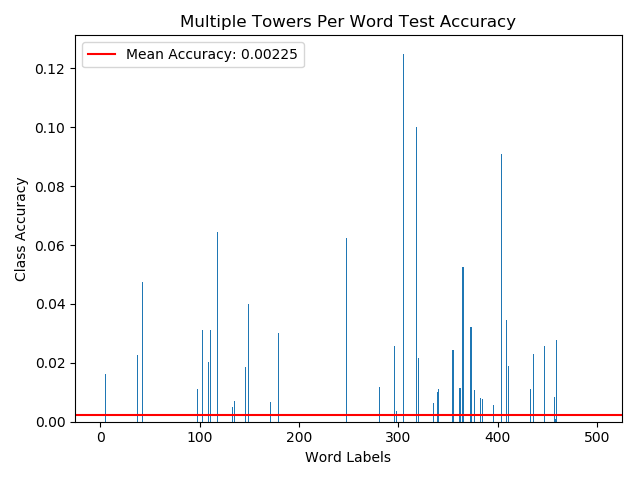
\includegraphics[width=\textwidth]{figures/gan/multiple_towers_acc.png}
        \caption{Multiple Towers}\label{fig:gan_multi_towers}
    \end{subfigure}
    \begin{subfigure}[b]{0.49\textwidth}
        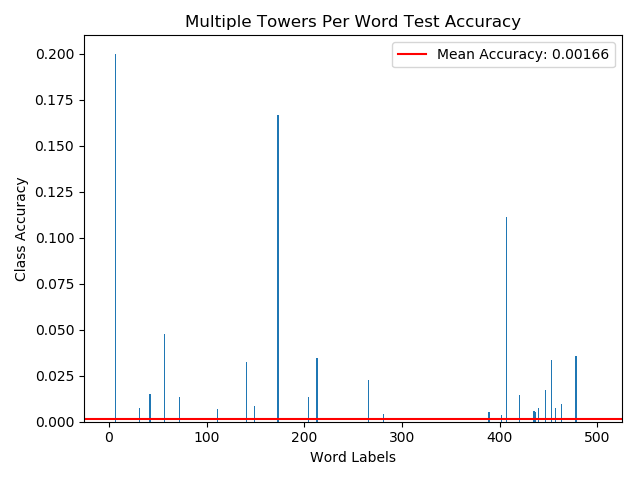
\includegraphics[width=\textwidth]{figures/gan/channels_acc.png}
        \caption{Blendshape Channels}\label{fig:gan_blendshape_channels}
    \end{subfigure}
    \caption{Classification Class Accuracy for Generated Data}\label{fig:gan_class_acc}
\end{figure}

While the pretrained classification models did not identify any speech features corresponding to the word labels in the generated samples, this does not definitively mean that the data is completely uncorrelated to the speech, just that the features which the classifiers have learnt to identify are not present.
To further investigate if there exists some correlation in the data, the two classification models have been retrained on the synthetic data.
The results however, confirm that there seems to be no correlation across the synthetically generated data.
Figure \ref{fig:gan_classification_synth_losses} demonstrates that both the Blendshape Channels and Multiple Towers models fail to generalise to unseen data completely, only able to learn features related to the training data.
The prediction accuracy further highlights this in Figure \ref{fig:gan_classification_synth_acc}, as accuracy on the validation data remains at 0.002 throughout training, equivalent to random guessing.

\begin{figure}[h!]
    \centering
    \begin{subfigure}[b]{0.49\textwidth}
        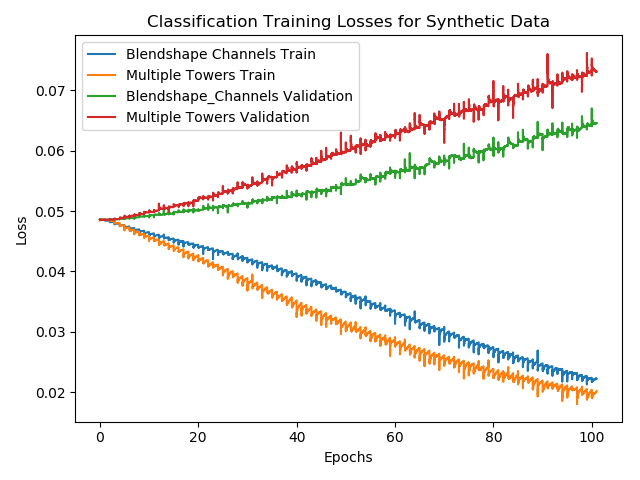
\includegraphics[width=\textwidth]{figures/gan/classification_losses.png}
        \caption{Training Losses}\label{fig:gan_classification_synth_losses}
    \end{subfigure}
    \begin{subfigure}[b]{0.49\textwidth}
        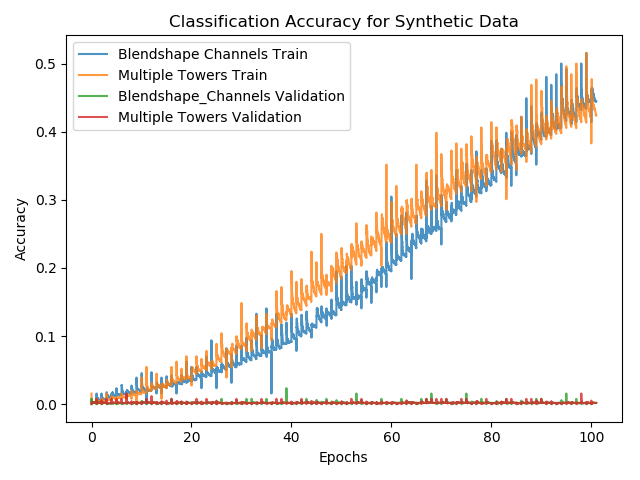
\includegraphics[width=\textwidth]{figures/gan/classification_acc.png}
        \caption{Training Accuracy}\label{fig:gan_classification_synth_acc}
    \end{subfigure}
    \caption{Classification Models Trained on Generated Data}\label{fig:gan_synth_classification}
\end{figure}

\section{Conclusions}
This chapter has discussed the use of a GAN model to generate synthetic Blendshape Parameters given an audio input upon which to drive a model.
The audio was represented by the use of MFCC values, which was combined with noise as an input to the Generator model.
The Critic was input with audio in the same MFCC representation on which the Generator was trained and corresponding Blendshape Parameter values from the original dataset and generated Blendshape Parameters from the Generator.
The Critic learnt to distinguish the real pairing of Blendshape Parameters and audio from the fake successfully, while the Generator attempted to learn to produce realistic Blendshape Parameters to fool the Critic.

While the generated samples appeared to be correlated with the audio to a human observer, evaluation of the pretrained classification models from Chapter \ref{chap:classification} highlighted that there was no correlation between the generated Blendshape Parameters and the words spoken in the audio samples.
This further highlights the difficulties of lip reading as a task for humans while the use of Blendshape Parameters for prediction is possible for a machine learning model.
